\documentclass[12pt]{article}

%opening
\title{Unimathematik für Informatikstudiengänge \\ Zusammenfassung}
\author{Konstantin Lukas}
\date{Fassung vom 03.08.2021}
\usepackage{amsmath,amsfonts,amssymb,amsthm}
\usepackage{braket}
\usepackage[margin=2cm]{geometry}
\usepackage{bbold}
\usepackage{etoc}
\usepackage{blindtext}
\usepackage{tikz}
\usepackage{array}
\usepackage[most]{tcolorbox}
\usepackage{hyperref }
\usepackage{pgfplots}
\DeclareRobustCommand{\bigfrac}[3][5pt]{%
	\frac{\hspace{#1}#2\hspace{#1}}{\hspace{#1}#3\hspace{#1}}}

\begin{document}
\maketitle
\tableofcontents
\etocsettocstyle{\noindent\rule{\linewidth}{.4pt}}

\section{Mengen}
\subsection{Vereinigung}
	\begin{flalign*}
		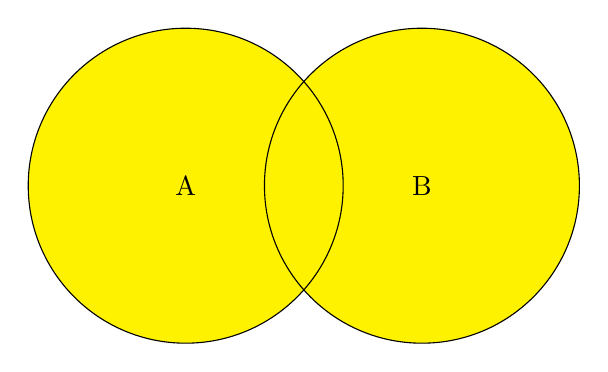
\begin{tikzpicture}
		\fill[yellow] (3,0) circle (2cm);
		\fill[yellow] (0,0) circle (2cm);
		\draw (0,0) circle (2cm);
		\draw (3,0) circle (2cm);
		\draw (0,0) node {A};
		\draw (3,0) node {B};
		\end{tikzpicture}&&
	\end{flalign*}
	\begin{flalign*}
		A \cup B := \{x \mid x \in A \: oder \: x \in B\}&&
	\end{flalign*}
\subsection{Durchschnitt}
	\begin{flalign*}
		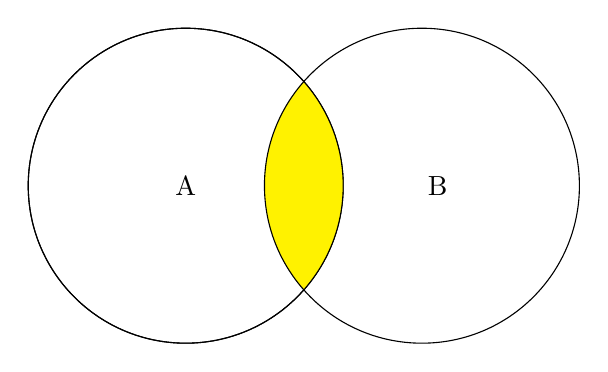
\begin{tikzpicture}
		\begin{scope}
			\draw [clip](0,0) circle (2cm);
			\fill[yellow] (3,0) circle (2cm);
		\end{scope}
		\draw (0,0) circle (2cm);
		\draw (3,0) circle (2cm);
		\draw (0,0) node {A};
		\draw (3.2,0) node {B};
		\end{tikzpicture}&&
	\end{flalign*}
	\begin{flalign*}
		A \cap B := \{x \mid x \in A \: und \: x \in B\}&&
	\end{flalign*}
\subsection{Differenz}
	\begin{flalign*}
		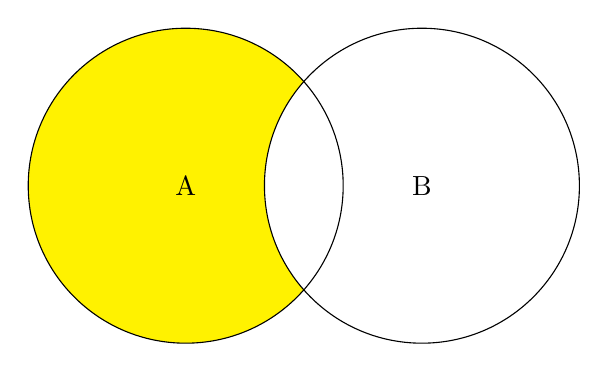
\begin{tikzpicture}
		\begin{scope}
			\fill[yellow] (0,0) circle (2cm);
			\clip (3,0) circle(2cm);
			\fill[white] (3,0) circle (2cm);
		\end{scope}
		\draw (0,0) circle (2cm);
		\draw (3,0) circle (2cm);
		\draw (0,0) node {A};
		\draw (3,0) node {B};
		\end{tikzpicture}&&
	\end{flalign*}
	\begin{flalign*}
		A \setminus B := \{x \mid x \in A \: und \: x \notin B\}&&
	\end{flalign*}
\subsection{Symmetrische Differenz}
	\begin{flalign*}
		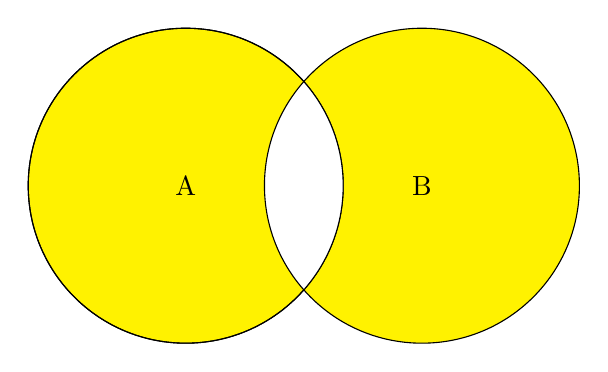
\begin{tikzpicture}
			\fill[yellow] (0,0) circle (2cm);
			\fill[yellow] (3,0) circle (2cm);
			\begin{scope}
				\draw [clip](0,0) circle (2cm);
				\fill[white] (3,0) circle (2cm);
			\end{scope}
			\draw (0,0) circle (2cm);
			\draw (3,0) circle (2cm);
			\draw (0,0) node {A};
			\draw (3,0) node {B};
			\end{tikzpicture}&&
		\end{flalign*}
	\begin{flalign*}
		A \triangle B := \{ x \mid (x \in A) \: \veebar \: ( x \in B ) \}&&
		A \triangle B := \{ x \mid (x \in A) \: \nleftrightarrow \: ( x \in B ) \}&&
	\end{flalign*}
\subsection{Definierte Zahlenmengen}
Natürliche Zahlen
	\begin{flalign*}
		\mathbb{N} = \{ 1; 2; 3; ... \}&&
	\end{flalign*}\newline
Menge der Natürliche Zahlen
	\begin{flalign*}
		\mathbb{N}_0 = \{ 0; 1; 2; 3; ... \}&&
	\end{flalign*}\newline
Ganze Zahlen
	\begin{flalign*}
		\mathbb{Z} = \{ ... ; -2; -1; 0; 1; 2; 3; ... \}&&
	\end{flalign*}\newline
Rationale Zahlen
	\begin{flalign*}
		\mathbb{Q} = \left\{ \frac{p}{q} \mid p, q \in \mathbb{Z}, q \neq 0 \right\}&&
	\end{flalign*}\newline
	Reelle Zahlen\newline
	Die reellen Zahlen umfassen die rationalen Zahlen und die irrationalen Zahlen.\newline\newline
	Irrationale Zahlen
	\begin{flalign*}
		\mathbb{R} \setminus \mathbb{Q}&&
	\end{flalign*}
\section{Betrag}
	\begin{flalign*}
		\vert a \vert = \left\{ a \atop -a \right. \;\;&
		a \ge 0 \atop a < 0 &
	\end{flalign*}
	\begin{flalign*}
		\vert -a \vert = \vert a \vert&&
	\end{flalign*}
\section{Intervalle}
	\subsection{Abgeschlossene Intervalle}
		$[a;b] := \{ x \in \mathbb{R} \mid a \le x \le b \}$
	\subsection{Offene Intervalle}
		$(a;b) = \: ]a;b[ \: := \{ x \in \mathbb{R} \mid a < x < b \}$
	\subsection{Halboffene Intervalle}
		Rechtsoffen \newline
		$[a;b) = \: [a;b[ \: :=  \{ x \in \mathbb{R} \mid a \le x < b \}$ \newline\newline
		Linksoffen \newline
		$(a;b] = \: ]a;b] \: :=  \{ x \in \mathbb{R} \mid a < x \le b \}$
\section{Binomische Formeln}
	$(a+b)^2 = a^2 + 2ab + b^2$ \newline\newline
	$(a-b)^2 = a^2 - 2ab + b^2$ \newline\newline
	$(a+b)(a-b) = a^2 - b^2$
\section{Euklidischer Algorithmus}
	Der euklidische Algorithmus findet den größten gemeinsamen Teiler zweier Zahlen. Das eignet sich ausgezeichnet dazu, Brüche zu kürzen. Der vorletzte Rest bevor $R = 0$ eintritt, ist das Ergebnis.
	\begin{flalign*}
		& 2160 : 2592 = 0 \;\;\; R = 2160 \\
		& 2592 : 2160 = 1 \;\;\; R = 432 \\
		& 2160 : 432 = 5 \;\;\; R = 0 &&
	\end{flalign*}
	\begin{flalign*}
	\frac{2592}{2160} = \frac{6 \cdot 432}{5 \cdot 432} = \frac{6}{5}&&
	\end{flalign*}
\section{Brüche dividieren}
	Um zwei Brüche zu dividieren bildet man den Kehrwert vom Divisor und multipliziert diesen mit dem Dividend.
	\begin{flalign*}
	\frac{p_1}{q_1} : \frac{p_2}{q_2} = \frac{p_1}{q_1} \cdot \frac{q_2}{p_2}&&
	\end{flalign*}
	\begin{flalign*}
	\bigfrac {\frac{p_1}{q_1}}  {\frac{p_2}{q_2}} = \frac{p_1}{q_1} \cdot \frac{q_2}{p_2}&&
	\end{flalign*}
\section{Potenzgesetze}
	\begin{tcolorbox}[boxsep=0pt,top=.5cm,left=1cm,right=1cm, bottom=.8cm,arc=0pt,auto outer arc,colback=white,colframe=black, enlarge top by=.25cm, enlarge bottom by=.25cm]
		\begin{flalign*}
			& a^k \cdot a^m = a^{k+m} \\\\
			& \cfrac{b^k}{b^m} = b^{k-m} \\\\
			& a^k \cdot b^k = (a \cdot b)^k \\\\
			& \cfrac{a^k}{b^k} = \left( \frac{a}{b} \right)^k \\\\
			& (a^k)^m = a^{k \cdot m} && 
		\end{flalign*}
	\end{tcolorbox}
	Für $a>0$ und jede rationale Zahl $\frac{p}{q}$ (mit $p,q \in \mathbb{Z}$ und $q>0$) ist
	\begin{flalign*}
	a^{\frac{p}{q}} = \sqrt[q]{a^p} = (\sqrt[q]{a})^p && 
	\end{flalign*}
	Beispiel: Bestimmen Sie $m$ und $n$ so, dass gilt: $(9x^7)^2 = mx^n$
	\begin{flalign*}
		(9x^7)^2 = mx^n \\
		81x^{14} = mx^n &&
	\end{flalign*}
	$m = 81$ und $n = 14$
\section{Wurzelgesetze}
	\begin{tcolorbox}[boxsep=0pt,top=1cm,left=1cm,right=1cm, bottom=1cm,arc=0pt,auto outer arc,colback=white,colframe=black, enlarge top by=.25cm, enlarge bottom by=.25cm]
		Für $a,b,c \in \mathbb{R}$ mit $a,b \ge 0, c > 0$ und $m, n \in \mathbb{N}$ gilt
		\begin{flalign*}
			& \sqrt[n]{ab} = \sqrt[n]{a} \cdot \sqrt[n]{b} \\\\
			& \sqrt[n]{\frac{a}{c}} = \frac{\sqrt[n]{a}}{\sqrt[n]{c}} \\\\
			& \sqrt[n]{\sqrt[m]{a}} = \sqrt[n \cdot m]{a} && 
		\end{flalign*}
	\end{tcolorbox}
	Beispiel 1: Nach der dritten Binomischen Formel gilt für $a,b > 0, a \neq b$:
	\begin{flalign*}
	& \cfrac{1}{\sqrt{a}+\sqrt{b}} & \cdot (\sqrt{a}-\sqrt{b}) && \\
	= & \cfrac{\sqrt{a}-\sqrt{b}}{(\sqrt{a}+\sqrt{b})(\sqrt{a}-\sqrt{b})} \\ 
	= & \cfrac{\sqrt{a}-\sqrt{b}}{\sqrt{a}^2-\sqrt{b}^2} \\ 
	= & \cfrac{\sqrt{a}-\sqrt{b}}{a-b} &&
	\end{flalign*}
	\hrulefill\newline\newline
	Beispiel 2:
	\begin{flalign*}
	& \frac{\sqrt{(1+a^2) \cdot (a-b)^2}}{\sqrt[4]{16(1+a^2)^2}} \\
	= & \sqrt{\frac{(1+a)^2 \cdot (a-b)^2}{\sqrt{16(1+a^2)^2}}} \\ 
	= & \sqrt{\frac{(1+a)^2 \cdot (a-b)^2}{4(1+a)^2}} \\ 
	= & \frac{1}{2}\sqrt{(a-b)^2} \\ 
	= & \frac{\mid a-b \mid}{2} &&
	\end{flalign*}
	\subsection{Wurzeltherme vereinfachen (Beispiele)}
		\begin{flalign*}
			\sqrt{2}+\dfrac{2}{2\sqrt{2}+3} & = \dfrac{}{}\sqrt{2}+\dfrac{ 2\cdot ( 2\sqrt{2}-] ) }{\left( 2\sqrt{2}+3\right) \left( 2\sqrt{2}-3\right) } \\
			& = \sqrt{2}+\dfrac{4\sqrt{2}-6}{\left( 2\sqrt{2}\right) ^{2}-3^{2}} \\
			& = \sqrt{2}+\dfrac{4\sqrt{2}-6}{-1} \\
			& = \sqrt{2}-4\sqrt{2}+6 \\
			& = 6-3\sqrt{2} &&
		\end{flalign*}
		\hrulefill
		\begin{flalign*}
		\dfrac{1}{\sqrt{1+x^{2}}-1}-\dfrac{1}{\sqrt{1+x^{2}}+1} & = \dfrac{\sqrt{1+x^{2}}+1}{\left( \sqrt{1+x^{2}}-1\right) \cdot \left( \sqrt{1+x^{2}}+1\right) } - \dfrac{\sqrt{1+x^{2}}-1}{\left( \sqrt{1+x^{2}}+1\right) \cdot \left( \sqrt{1+x^{2}}-1\right) } \\
		& = \dfrac{\left( \sqrt{1+x^{2}}+1\right) -\left( \sqrt{1+x^{2}}-1\right) }{1+x^{2}-1} \\
		& = \frac{2}{x^2} &&
		\end{flalign*}
		\hrulefill\newline\newline
		Beispiel 3: Bestimmen Sie $x$ und $y$, sodass $\frac{x}{y}$ vollständig gekürzt ist.
		\begin{flalign*}
			\dfrac{2\cdot 2^{\frac{5}{2}}}{2^{\frac{1}{4}}}=2^{\frac{x}{y}} \\
			2 \cdot \dfrac{2^{\frac{5}{2}}}{2^{\frac{1}{4}}}=2^{\frac{x}{y}} \\
			2 \cdot 2^{\frac{5}{2}-\frac{1}{4}} = 2^{\frac{x}{y}} \\
			2 \cdot 2^{\frac{9}{4}} = 2^{\frac{x}{y}} \\
			2^{\frac{13}{4}} = 2^{\frac{x}{y}} &&
		\end{flalign*}
		Damit gilt $x = 13$ und $y = 4$.
\section{Lösungsmenge}
	Beispiel 1 ($x^2=-1$):\newline
	$\mathbb{L} = \emptyset$ \newline\newline
	Beispiel 2 ($x^2 = 4$):\newline
	$\mathbb{L} = \{-2;2\}$\newline\newline
	Beispiel 3 ($sin(x) = 0$):\newline
	$\mathbb{L} = \{...;-2\pi;-\pi;0;\pi;2\pi; ...\}$\newline\newline
	Beispiel 4 ($x^2 + y = 5$):\newline
	$\mathbb{L} = \{(x_0;y_0)\in\mathbb{R}^2\mid x^2_0 + y_0 = 5\} = \{(x_0;5-x^2_0) \mid x_0\in\mathbb{R}^2\}$\newline\newline
	In diesem Fall ist die Lösungsmenge die Funktion $y=5-x^2$.\newline\newline
	\begin{tikzpicture}
		\begin{axis}[
			domain=-10:10,
			xmin=-10, xmax=10,
			ymin=-10, ymax=10,
			samples=200,
			axis y line=center,
			axis x line=middle,
			]
			\addplot+[mark=none] {5-x^2};
		\end{axis}
	\end{tikzpicture}
\section{Normalform}
	Eine Gleichung in der Form $ax^2+bx+c=0$ mit $a\neq0$ und $b,c\in \mathbb{R}$, heißt quadratisch. Spezial bezeichnet man $x^2+px+q=0$ mir $p,q\in \mathbb{R}$, als quadratische Gleichung in Normalform.\newline\newline
	Man kann eine quadratische Gleichung in die Normalform überführen, indem man durch $a$ teilt: $x^2+\frac{b}{a}x+\frac{c}{a}=0$.
	\subsection{p-q-Formel}
	\label{subsec:pqformel}
	\begin{tcolorbox}[boxsep=0pt,top=1cm,left=1cm,right=1cm, bottom=.75cm,arc=0pt,auto outer arc,colback=white,colframe=black, enlarge top by=.25cm, enlarge bottom by=.25cm]
	Um die Nullstellen einer quadratischen Gleichung in der Normalform zu finden, kann man die p-q-Formel benutzen: $x_{\pm}=-\frac{p}{2}\pm\sqrt{\left(\frac{p}{2}\right)^2-q}$.
	\end{tcolorbox}
	\noindent$D=\left(\frac{p}{2}\right)^2-q$ ist die Diskriminante. Sie gibt Aufschluss über die Lösungsmenge.
	\begin{flalign*}
	&D>0\Rightarrow Es\;gibt\;zwei\;Lsg.\\
	&D=0\Rightarrow Es\;gibt\;eine\;Lsg.\\
	&D<0\Rightarrow Es\;gibt\;keine\;Lsg.&&
	\end{flalign*}
\section{Quadratische Ergänzung}
	\begin{tcolorbox}[boxsep=0pt,top=.75cm,left=1cm,right=1cm, bottom=.65cm,arc=0pt,auto outer arc,colback=white,colframe=black, enlarge top by=.25cm, enlarge bottom by=.25cm]
		Die äquivalente Umformung der quadratischen Gleichung in Normalform $x^2+px+q=0$ in $\left(x+\frac{p}{2}\right)^2=-q+\left(\frac{p}{2}\right)^2$ wird als quadratische Ergänzung bezeichnet. In anderen Worten fügt man den Term $+\left(\frac{p}{2}\right)^2-\left(\frac{p}{2}\right)^2$ hinzu.
	\end{tcolorbox}
	\noindent Beispiel:
		\begin{flalign*}
	x^2+8x+7 &= 0\\
	x^2+8x+\left(\frac{8}{2}\right)^2+\left(\frac{8}{2}\right)^2+7 &= 0\\
	x^2+8x+4^2+4^2+7 &= 0\\
	(x+4)^2+4^2+7 &= 0\\
	(x+4)^2-9 &= 0\;\;\;\;\;\;\;\;\;\mid+9\\
	(x+4)^2 &= 9\;\;\;\;\;\;\;\;\;\mid\sqrt{\ }\\
	x&=\pm\sqrt{9}-4\\
	\mathbb{L}&=\{-1;-7\}&&
	\end{flalign*}
\section{Faktorisieren}
	Um die Nullstellen eines Terms zu finden, bietet es sich an, ihn als Produkt einfacher Terme zu schreiben, denn ist ein Faktor $0$, ist das Produkt ebenfalls $0$. Den Term in so eine Form zu überführen, nennt sich Faktorisieren.
	\subsection{Faktorisierung durch Ausklammern}
		Beispiel:
		\begin{flalign*}
			x^4+2x^3+3x^2 &= 0\\
			x^2(x^2+2x+3) &= 0\\
			x^2 &= 0\;oder\;(x^2+2x+3) = 0\\
			\mathbb{L} &= \{0\}&&
		\end{flalign*}
		Für $x^2+2x+3 = 0$ existiert keine reelle Lösung (s. \nameref{subsec:pqformel}).
	\subsection{Faktorisierung mit binomischen Formeln}
		Beispiel:
		\begin{flalign*}
		9x^2+30x+25& = 0\\
		(3x+5)^2& = 0\\
		3x+5&=0\;\;\;\;\;\;\;\;\;\mid-5\\
		3x&=-5\;\;\;\;\;\;\;\;\;\mid:3\\
		x&=-\frac{5}{3}\\
		\mathbb{L}&=\left\{-\frac{5}{3}\right\}&&
		\end{flalign*}
	\subsection{Faktorisierung mit dem Satz von Viëta}
		\begin{tcolorbox}[boxsep=0pt,top=.75cm,left=1cm,right=1cm, bottom=.65cm,arc=0pt,auto outer arc,colback=white,colframe=black, enlarge top by=.25cm, enlarge bottom by=.25cm]
		Der Satz von Viëta besagt, dass $x^2+px+q=(x-x_1)\cdot(x-x_2)$ ist. $p$ und $q$ lassen sich auf die Nullstellen zurückführen: $x_1+x_2=-p$ und $x_1\cdot x_2 = q$.
		\end{tcolorbox}
		\noindent Daraus lässt sich $x_2=\frac{q}{x_1}$ ableiten. Wenn man also durch Raten eine Nullstelle findet, kann man so die andere Nullstelle auch ganz einfach finden.\newline\newline
		Beispiel (eine Nullstelle ist $1$, die andere ergibt sich als $\sqrt{2} = \frac{\sqrt{2}}{1}$):
		\begin{flalign*}
			x^2+(\sqrt{2}-1)x-\sqrt{2}&=0\\
			(x-1)\cdot (x+\sqrt{2})&=0\\
			\mathbb{L}=\{1;-\sqrt{2}\}&&
		\end{flalign*}
\end{document}
